

\begin{comment}
\section{Electrochemical analyzer}
On top of the microscope, another machine is used in the set up that changes the potential electrochemically: an electrochemical analyzer (Model 800B Series Electrochemical Detector, CH Instruments). A 0.25 mm thin golden wire acts as working electrode. One end is connected to the electrochemical analyzer while the other end touches the functionalised surface. The counter electrode is a 0.5mm thin platinum wire (company where we bought it) and is sufficient deep in the solution that it acts as a counter electrode but it does not touch the glass surface. The reference electrode is a saturated calomel electrode (SCE) and does not touch the surface neither but yet is deep enough in the solution. Both the counter and the reference electrode are connected to the electrochemical analyzer. These three electrodes together form the electrochemical cell.



\subsection*{Electron mediator}
An electrochemical interface consist of an electrode and an electrolyte. The potential is the energy per unit charge required to take a charge from one side of the interface to the other. This electrode potential is related to chemical activities of the electrochemical reaction by the Nernst equation (Equation \ref{nernst}). When an electrode-electrolyte interface is at equilibrium - that is it is at its standard potential - no net reaction occurs at the interface. This equilibrium is violated when a current flow due to application of an external potential. The flow or changes across the electrode-electrolyte interface will induce a change in potential of the electrode. This change is described by the Butler-Volmer equation \cite{Shinwari2010}. 

The midpoint potential of the proteins is around $-270 mV$, therefore an electron mediator with potentials around the proteins' midpoint potential are necessary.

\subsection*{potassium ferricyanide/potassium ferrocyanide}
With a midpoint potential of $-237 mV$, the redox couple potassium ferricyanide ($[\textup{Fe(CN)}_{6}]^{4-}$)/ferrocyanide ($[\textup{Fe(CN)}_{6}]^{3-}$) would have been the perfect electron mediator for this experiment. To see what range of different potentials can be reached with this redox couple, several cy. The oxidation of ferrocyanide, resulting in ferricyanide is given by
\begin{equation}
[\textup{Fe(CN)}_{6}]^{4-}\rightleftharpoons[\textup{Fe(CN)}_{6}]^{3-} + \textup{e}^{-}.
\end{equation}
This reaction is reversible. When applying different currents, the potential was not reached over the whole spectrum. The oxidation of ferrocyanide was easy: high potentials were reached in short times (1-5 minutes) (pictures). However, reducing the ferricyanide was only possible to a certain extend. The process was extremely slow, it took hours to go below -200 mV (aanpassen). . By removing the oxygen, the potassium ferricyanide/potassium ferrocyanide redox couple should do it. This was however practically impossible for the set up.

\end{comment}

\subsection*{phenazine ethosulfate (PES}



\begin{enumerate}
\item \textbf{0.1mM phenazine ethosulfate (PES) using 30 nm thick golden layer with cross-transparent area glass slides with HEPES (pH = 7) as buffer}. The first check to see a difference in potential is to apply the two extremes. A cycle is in this context meant as going from the +mV to the same amount in -mV. The first few cycles looked promising (see Figure ). Considered that for each small area of proteins the potential has to be changed around 20 times in order to get a decent spectrum of different potentials, the set up should work for a lot of cycles. However, after 3-4 cycles the difference between +300mV and -300mV were considerable less (see Figure ). What stood out was the fact that after several hours of experimenting, the gold on the glass slide came loose. This was visible on the images of the borders too (see Figure \ref{damaged_border}. The explanation for this is that the PES is damaging the gold. Applying a bit less potential would make the gold survive a few more cycles, but not sufficient enough to do proper research. This problem, as mentioned in the next two points, could be solved in two different ways: (1) a protective layer on top of the gold so the PES can't damage the gold or (2) making a thicker gold layer so it takes more time for PES to damage the gold.

\item \textbf{0.1mM phenazine ethosulfate (PES) using 30nm thick protected golden layer with cross-transparent area glass slides with HEPES (pH = 7) as buffer}. To protect the gold, a thin layer of hydroxyl surface, $\textup{HSC}_{8}\textup{OH}$ and $\textup{HSC}_{6}\textup{OH}$ were applied on the gold. This should protect the gold from PES reaching the gold surface. Previous studies have shown, despite this layer on the gold, that electron transfer occurs \cite{Ciobanu2006}. For the first slide,  $\textup{HSC}_{6}\textup{OH}$ was mixed in water and rested on top of the gold for around 2 hours. This resulted in a lot of impurities on the transparent areas (see Figure ) which made it impossible to see the single molecules. A reason for this could be that $\textup{HSC}_{6}\textup{OH}$ is hydroxyl and doesn't mix well with water. For the second slide, $\textup{HSC}_{8}\textup{OH}$ was mixed in oil and rested on the sample slide overnight. The impurities, as can be seen in Figure X, were still present but in lesser extend. Also the redox switching was not as good as it needed to be. 

This resulted in the later option: increasing the gold thickness.
\item \textbf{0.1mM phenazine ethosulfate (PES) using 200nm thick golden layer with cross-transparent area glass slides with HEPES (pH = 7) as buffer}. The increase of the thickness of the golden layer would lead to the PES taking much longer to damage the gold to a point where redox reactions would be affected. However, when images were taken, almost no proteins were present near the borders (see Figure \ref{no_prot}). This is most likely the result of the sputtering machine. During this process, gold particles manage to get under the iron crosses, resulting in a very thin layer (Figure \ref{goldborderillu}). This thin layer of gold has a very high transparency (a 5nm thin layer of gold has a transparency of over 80\% \cite{Kossoy2015}), which makes this layer not visible under the microscope. Far away from the border, the protein density recovers to the expected one, but almost no redox reactions take place because it is too far away from the golden layer (working electrode).



\begin{figure}
\begin{subfigure}{.5\textwidth}
  \centering
  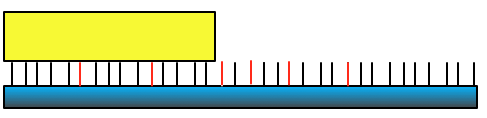
\includegraphics[width=.7\linewidth]{ideal_case}
  \label{}
\end{subfigure}%
\begin{subfigure}{.5\textwidth}
  \centering
  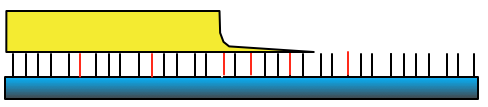
\includegraphics[width=.7\linewidth]{realistic_case}
  \label{}
\end{subfigure}
\caption{Illustration of the golden layer on top of the glass surface, not on scale. The red lines represent biotin. In the ideal case (left) the border is vertical and biotin near the surface will be occupied by proteins. In the case of 200nm golden layer, a very thing golden layer prevents the protein to bind to the glass surface near the border. }
\label{goldborderillu}
\end{figure}

\item \textbf{A \diameter250 $\upmu \textup{m}$ golden wire with a small weight using an immobilised transparent glass slide in a mixture of PES and HEPES (pH = 7) as buffer}. Since using the gold layer was to no avail, a new idea came to mind to use a small weight to bring a golden wire to the surface. By imaging this proteins near this wire, redox reaction are visible. 

\end{enumerate} 
